% This report follows the original Springer LNCS project template.
\documentclass[runningheads]{llncs}
%
% Preserve Vietnamese support where installed; this English report also builds
% on TeX installations without the optional vietnam package.
\IfFileExists{vietnam.sty}{\usepackage[utf8,nocaptions]{vietnam}}{\usepackage[utf8]{inputenc}}
\usepackage{graphicx}
\usepackage{booktabs}
\usepackage{tabularx}
\usepackage{url}
\usepackage{tikz}
\usepackage{float}
\usetikzlibrary{arrows.meta}
% Shared visual language for the three DPE hypothesis diagrams.
\definecolor{dpeland}{HTML}{A65320}
\definecolor{dpewater}{HTML}{216B9B}
\definecolor{dpeink}{HTML}{263747}
\tikzset{
  dpe diagram/.style={font=\sffamily\scriptsize, text=dpeink,
    >=Stealth, line width=0.55pt},
  dpe land/.style={circle, draw=dpeland, fill=dpeland!12,
    text=dpeland, minimum size=5.5mm, inner sep=1pt},
  dpe water/.style={rectangle, draw=dpewater, fill=dpewater!12,
    text=dpewater, minimum size=5.5mm, inner sep=1pt},
  dpe box/.style={draw=dpeink!45, rounded corners=2pt,
    fill=dpeink!3, align=center, inner sep=4pt},
  dpe arrow/.style={->, draw=dpeink!75},
  dpe heading/.style={font=\sffamily\scriptsize\bfseries}
}
%
\begin{document}
%
\title{Background Shortcut Learning Mitigation for Waterbirds}
%
\titlerunning{Waterbirds Baseline Reproduction}
%
\author{Chau Tan Phat\inst{1,2} \and
Nguyen Dang Khang\inst{1,2} \and
Nguyen Phu Trong\inst{1,2} \and
Nguyen Dinh Minh Huy\inst{1,2}}
%
\authorrunning{C. T. Phat, N. D. Khang, N. P. Trong, N. D. M. Huy}
%
\institute{Faculty of Information Technology, University of Science, Ho Chi Minh City, Vietnam \and
Vietnam National University, Ho Chi Minh City, Vietnam\\
\email{ctphat2519@apcs.fitus.edu.vn, ndkhang2535@apcs.fitus.edu.vn}\\
\email{nptrong2530@apcs.fitus.edu.vn, ndmhuy2521@apcs.fitus.edu.vn}}
%
\maketitle
%
\begin{abstract}
This is our weekly report on three methods that try to stop image classifiers from relying on the background: DPE, POTER, and AutoBackSwap. We ran each method on the Waterbirds dataset and compared our numbers with the ones in the papers. DPE and AutoBackSwap came close to the published worst-group accuracy. POTER finished training for one seed, but we only have validation results so far. While looking at AutoBackSwap's mistakes, we found that three bird species seem to be labeled wrongly in the dataset, and that they cause many of its errors. We also evaluate the head-reweighting hypothesis for DPE over three training seeds. Validation-selected weighting did not improve worst-group accuracy over matched uniform averaging; two other DPE hypotheses remain untested.

\keywords{Shortcut learning \and Waterbirds \and Reproducibility \and Worst-group accuracy.}
\end{abstract}
%
\section{Introduction}
\subsection{Problem statement}
\paragraph{Definition.}
Each image in the Waterbirds dataset \cite{waterbirds} shows a bird, and the task is to decide whether it is a landbird or a waterbird. The difficulty is that the background is correlated with the label: most landbirds are photographed on land and most waterbirds on water. A model can therefore get good accuracy just by looking at the background, without looking at the bird.

\paragraph{Why it is hard.}
A normally trained model (ERM, which simply minimizes the average training loss) tends to learn this shortcut. It then fails on the rare images where the background is misleading, such as a landbird on water. In practice we also do not know which group an image belongs to during training, which makes the problem harder.

\subsubsection{Research scope}
We re-ran three existing methods on Waterbirds, compared our results with the papers, and investigated their errors. We subsequently tested whether reweighting frozen DPE heads improves worst-group accuracy.

\subsection{Literature review}
The three methods we study take different approaches. POTER \cite{poter} gives more weight to training images that look like the hard cases in a small validation set. DPE \cite{dpe} trains many small classifiers on top of a frozen model and averages them. AutoBackSwap \cite{autobackswap} cuts the bird out of each image and pastes it onto a different background, so the model cannot depend on the background.

\subsection{Contributions}
\begin{itemize}
    \item We ran DPE, POTER, AutoBackSwap, and an ERM baseline, and compared the results with the papers.
    \item We checked the individual test predictions of AutoBackSwap and ERM, and found a possible labeling problem in the dataset and a small bug in the released code.
    \item We formulated three DPE hypotheses and evaluated head reweighting (H2) using matched ensembles over seeds 0--2; prototype re-pairing (H1) and larger prototype subsets (H3) remain untested.
\end{itemize}

\section{Related Work}
ERM works well on average but is dominated by the majority groups. GroupDRO \cite{waterbirds} fixes this by directly improving the worst group, but it needs group labels for every training image. The three methods in this report try to avoid that requirement.

\section{Approach}
All three methods use a ResNet-50 pretrained on ImageNet.
\begin{itemize}
    \item \textbf{DPE} \cite{dpe}: first train the model with ERM and freeze it. Then train 15 small classifiers (we call them heads) on balanced subsets of the data, and average their predictions.
    \item \textbf{POTER} \cite{poter}: compare the training images with a small validation set whose groups are known, and give higher sampling weight to the images that are similar to the hard groups.
    \item \textbf{AutoBackSwap} \cite{autobackswap}: use a detector to find the bird, remove it and fill in the background, then paste the bird onto random backgrounds while training.
\end{itemize}

\section{Experiments}

\subsection{Dataset and Metrics}
We use the official Waterbirds splits \cite{waterbirds}: 4,795 training, 1,199 validation, and 5,794 test images. The images fall into four groups:
$G_1$ landbird on land (2,255 test images),
$G_2$ landbird on water (2,255),
$G_3$ waterbird on land (642), and
$G_4$ waterbird on water (642).
We report overall accuracy (Acc) and worst-group accuracy (WGA), which is the lowest accuracy among the four groups. Checkpoint and aggregation choices follow the documented method-specific protocol, without test-based selection. In the H2 study, the backbone uses its final epoch; head epochs and aggregation are selected using separate validation subsets.

\subsection{Settings}
The historical DPE runs used seed 0 in two versions: the standard one, and the enhanced one that uses a stronger ERM model (ERM$^*$). POTER was trained once (seed 1) for 300 epochs. AutoBackSwap and ERM were run on a Tesla T4 GPU: seeds 0--2 without minority-group training images, plus one AutoBackSwap run and three ERM runs with them. The subsequent H2 study uses three standard-track training seeds (0--2), with a separate validation allocation described below; its uniform ensembles are the matched controls for reweighting.

\subsection{Results and Discussion}
\subsubsection{Comparison with the papers}
Table~\ref{tab1} shows our results. DPE reached 89.00\% WGA in the standard setting (paper: 91.0$\pm$0.5\%) and 92.70\% in the enhanced setting (paper: 94.1$\pm$0.2\%), so we are about 2 points below the paper in both. For ERM and AutoBackSwap, our WGA is within two standard deviations of the paper in all four settings. Without minority-group images, AutoBackSwap raises WGA from 33.38\% (ERM) to 92.33\% (paper: 92.2\%). POTER finished training, and its best validation WGA is 90.10\% at epoch 258. This is a validation number, so we cannot compare it with the paper's test WGA of 90.9\% yet. We still need to recover the test results.

\begin{table}[t]
\centering
\caption{Results on Waterbirds (\%). Acc denotes overall accuracy and WGA denotes worst-group accuracy. DPE, ERM, and AutoBackSwap are evaluated on the held-out test split. POTER currently reflects validation metrics (epoch 258) for seed 1; held-out test evaluation is pending artifact recovery.}
\label{tab1}
\small
\setlength{\tabcolsep}{3.5pt}
\begin{tabular}{@{}lccccc@{}}
\toprule
Method and setting & Seeds & \multicolumn{2}{c}{Our result} & \multicolumn{2}{c}{Paper (Test)} \\
\cmidrule(lr){3-4}\cmidrule(l){5-6}
 & & Acc & WGA & Acc & WGA \\
\midrule
DPE, standard & 1 & 91.40 & 89.00 & 92.5$\pm$0.2 & 91.0$\pm$0.5 \\
DPE, enhanced ERM$^*$ & 1 & 93.30 & 92.70 & 96.0$\pm$0.1 & 94.1$\pm$0.2 \\
\midrule
POTER (val.\ checkpoint) & 1 & 91.60$^\dagger$ & 90.10$^\dagger$ & --- & 90.9$\pm$0.3 \\
\midrule
ERM, no minority & 3 & 68.68$\pm$1.00 & 33.38$\pm$1.51 & 68.4$\pm$1.9 & 33.4$\pm$4.4 \\
ERM, with minority & 3 & 93.67$\pm$0.23 & 78.45$\pm$2.22 & 93.6$\pm$0.4 & 74.9$\pm$3.3 \\
AutoBackSwap, no minority & 3 & 94.49$\pm$0.40 & 92.33$\pm$0.16 & 95.1$\pm$0.3 & 92.2$\pm$0.4 \\
AutoBackSwap, with minority & 1 & 95.44 & 92.37 & 95.0$\pm$0.5 & 93.0$\pm$0.9 \\
\bottomrule
\end{tabular}
\par\vspace{3pt}
{\footnotesize $^\dagger$Validation metrics at epoch 258 (held-out test evaluation pending recovery of test split logs).}
\end{table}

\subsubsection{Failure Case Analysis (AutoBackSwap)}
Recall the four groups: $G_1$ landbird on land, $G_2$ landbird on water, $G_3$ waterbird on land, and $G_4$ waterbird on water. We looked at the individual test predictions of ERM and AutoBackSwap (seed 0, no minority-group images). ERM makes 1,752 mistakes, mostly on $G_2$ and $G_3$ where the background is misleading (accuracy 34.90\% and 60.13\%). AutoBackSwap makes only 346 mistakes: 75 in $G_1$, 176 in $G_2$, 49 in $G_3$, and 46 in $G_4$.

We noticed three more things:
\begin{itemize}
    \item The released code prints the accuracies of $G_2$ and $G_3$ with their names swapped in \path{test_accuracies.txt}. After recomputing from \path{metadata.csv}, the real worst group is $G_2$ (92.20\%).
    \item 202 test images are misclassified in all three seeds, and 109 of them are in $G_2$. So the errors are not random.
    \item Three species (\path{102.Western_Wood_Pewee}, \path{021.Eastern_Towhee}, \path{088.Western_Meadowlark}; 90 test images) look like landbirds, but \path{metadata.csv} labels them as waterbirds. AutoBackSwap calls 64 of these 90 images landbirds, which gives 64 of its 346 mistakes and 37 of the 46 mistakes in $G_4$. These may be label errors in the dataset rather than model errors, but we have not verified this beyond looking at the species names.
\end{itemize}

\subsubsection{Ablation Study (DPE)}
In the standard setting, the full DPE gets 89.00\% WGA. Using random subsets without the covariance term gives 88.20\%, and using one fixed subset gives 88.80\%. So the full method is better by 0.2--0.8 points, which is a small gap from a single seed. In the enhanced setting all three variants give 92.70--92.80\%, so the differences are negligible.

\subsubsection{Observations and Hypotheses on DPE}
We formulated three hypotheses from the DPE aggregation procedure. H2 has now been evaluated using prediction caches and matched controls; H1 and H3 remain untested. Prediction disagreements are measured below, but no image-level attribution has established which heads rely on backgrounds.

\paragraph{Observation.} Each of the 15 DPE heads is a binary prototype classifier that holds exactly two prototypes, one per class. For an input feature, a head computes class probabilities from the distances to its own two prototypes only, and the final prediction is the uniform average of the 15 head probabilities. This design has three consequences: (i)~prototypes are only compared within their original pair, (ii)~every head contributes equally regardless of what it has learned, and (iii)~each head's decision uses only 2 of the 30 available prototypes.

\paragraph{H1: Shuffling prototype pairs across heads.} If the landbird prototype of one head is paired with the waterbird prototype of another head, does the resulting set of pairs introduce additional diversity into the ensemble and thereby improve WGA? Because the heads are trained on different balanced subsets, re-pairing yields new decision boundaries without additional training. We will compare random and exhaustive re-pairings on the trained heads, selecting the configuration by validation WGA.

\begin{figure}[H]
\centering
% Vector schematic; included from main.tex. Coordinates are in centimetres.
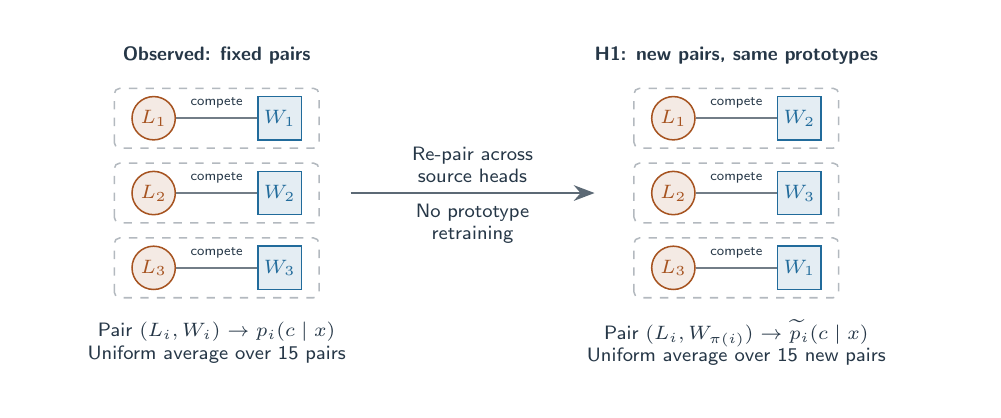
\begin{tikzpicture}[dpe diagram]
\path[use as bounding box] (-0.3,-4.15) rectangle (11.7,0.45);
\node[dpe heading] at (2.1,0.1) {Observed: fixed pairs};
\node[dpe heading] at (8.7,0.1) {H1: new pairs, same prototypes};
\foreach \i/\j/\y in {1/2/-0.7,2/3/-1.65,3/1/-2.6} {
  \draw[dashed,draw=dpeink!35,rounded corners=2pt]
    (0.8,\y-0.38) rectangle (3.4,\y+0.38);
  \node[dpe land] (l\i) at (1.3,\y) {$L_{\i}$};
  \node[dpe water] (w\i) at (2.9,\y) {$W_{\i}$};
  \draw[draw=dpeink!65] (l\i) -- (w\i)
    node[midway,above,font=\sffamily\tiny] {compete};
  \draw[dashed,draw=dpeink!35,rounded corners=2pt]
    (7.4,\y-0.38) rectangle (10,\y+0.38);
  \node[dpe land] (nl\i) at (7.9,\y) {$L_{\i}$};
  \node[dpe water] (nw\i) at (9.5,\y) {$W_{\j}$};
  \draw[draw=dpeink!65] (nl\i) -- (nw\i)
    node[midway,above,font=\sffamily\tiny] {compete};
}
\draw[dpe arrow,line width=1pt] (3.8,-1.65) -- (6.9,-1.65)
  node[midway,above,align=center] {Re-pair across\\source heads}
  node[midway,below,align=center] {No prototype\\retraining};
\node[align=center] at (2.1,-3.55)
  {Pair $(L_i,W_i)$ $\to$ $p_i(c\mid x)$\\Uniform average over 15 pairs};
\node[align=center] at (8.7,-3.55)
  {Pair $(L_i,W_{\pi(i)})$ $\to$ $\widetilde p_i(c\mid x)$\\Uniform average over 15 new pairs};
\end{tikzpicture}

\caption{H1: change which prototypes compete. Original DPE compares $L_i$ only with $W_i$. An example re-pairing compares $L_i$ with $W_{\pi(i)}$; each new pair still produces a two-class probability, and the ensemble still averages the pair probabilities. Circles denote landbird prototypes and squares waterbird prototypes; subscripts identify the source head. Only three of 15 pairs are shown. The prototypes stay fixed; whether the new comparisons improve WGA is untested.}
\label{fig:dpe-h1}
\end{figure}

\paragraph{H2: Reweighting the heads.}
Can validation-derived weights improve WGA over uniform $1/15$ probability averaging? Within each training seed, the backbone, features, 15 heads and test images are fixed; only aggregation changes. This tests a project adaptation, not an exact reproduction of the original DPE validation budget.

\begin{figure}[H]
\centering
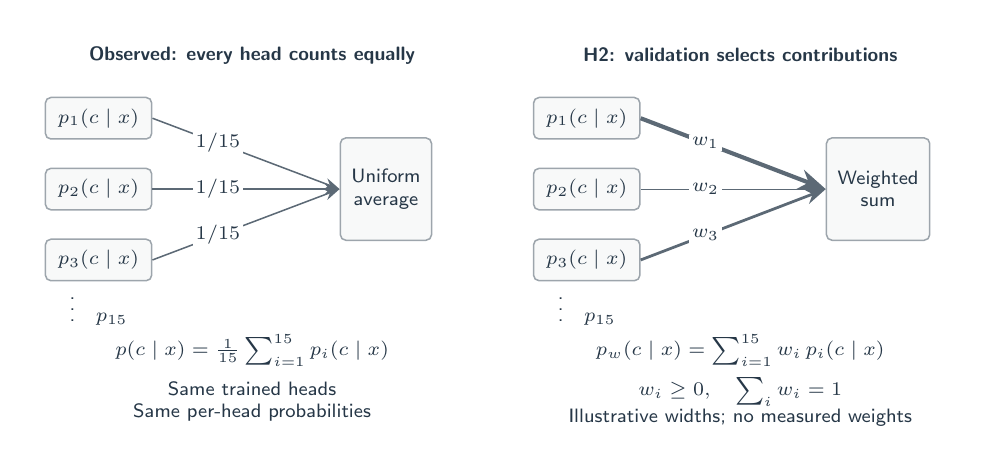
\begin{tikzpicture}[dpe diagram]
\path[use as bounding box] (-0.3,-4.65) rectangle (11.7,0.45);
\node[dpe heading] at (2.55,0.1) {Observed: every head counts equally};
\node[dpe heading] at (8.75,0.1) {H2: validation selects contributions};
\foreach \i/\y in {1/-0.7,2/-1.6,3/-2.5} {
  \node[dpe box,minimum width=1.35cm] (a\i) at (0.6,\y) {$p_{\i}(c\mid x)$};
  \node[dpe box,minimum width=1.35cm] (b\i) at (6.8,\y) {$p_{\i}(c\mid x)$};
}
\node[dpe box,minimum height=1.3cm] (avg) at (4.25,-1.6) {Uniform\\average};
\foreach \i in {1,2,3} {
  \draw[dpe arrow] (a\i.east) -- (avg.west)
    node[pos=0.35,fill=white,inner sep=1pt] {$1/15$};
}
\node[dpe box,minimum height=1.3cm] (weighted) at (10.5,-1.6) {Weighted\\sum};
\draw[dpe arrow,line width=1.5pt] (b1.east) -- (weighted.west)
  node[pos=0.35,fill=white,inner sep=1pt] {$w_1$};
\draw[dpe arrow,line width=0.4pt] (b2.east) -- (weighted.west)
  node[pos=0.35,fill=white,inner sep=1pt] {$w_2$};
\draw[dpe arrow,line width=1pt] (b3.east) -- (weighted.west)
  node[pos=0.35,fill=white,inner sep=1pt] {$w_3$};
\node at (0.6,-3.05) {$\vdots\quad p_{15}$};
\node at (6.8,-3.05) {$\vdots\quad p_{15}$};
\node at (2.55,-3.65) {$p(c\mid x)=\frac{1}{15}\sum_{i=1}^{15}p_i(c\mid x)$};
\node at (8.75,-3.65) {$p_w(c\mid x)=\sum_{i=1}^{15}w_i\,p_i(c\mid x)$};
\node[align=center] at (8.75,-4.3) {$w_i\geq 0,\quad\sum_i w_i=1$\\Illustrative widths; no measured weights};
\node[align=center] at (2.55,-4.3) {Same trained heads\\Same per-head probabilities};
\end{tikzpicture}

\caption{H2 compares uniform averaging with nonnegative weights summing to one, using the same frozen head probabilities. Unequal arrow widths are schematic. Weights are fitted and selected using validation data before test evaluation; unequal weights alone do not establish background dependence.}
\label{fig:dpe-h2}
\end{figure}

\paragraph{Protocol and experiment history.}
Validation subsets A, B and C contain 720, 241 and 238 images: A fits heads and selects their epochs, B fits weights, and C selects aggregation. All three training seeds share partition seed 0. Each standard-track backbone trains for 100 epochs without augmentation, then each of 15 heads trains for 20 epochs on a balanced 320-image A subset. The initial seed-0 power study produced identical C predictions for all 13 candidates, so uniform won. The expanded grid contains 20 candidates: uniform, 12 power rules, softmax with $\beta\in\{10,30\}$, top-$k$ with $k\in\{10,5\}$, and joint weighting with $\lambda\in\{1,0.1,0.01\}$. Joint fitting minimizes worst B-group negative log likelihood (NLL) plus $\lambda\| w-\mathbf{1}/15\|_2^2$ on the probability simplex. C selects by WGA, then overall accuracy; uniform wins complete ties and is available within every family. Only frozen winners and uniform are evaluated on test.

An initial multi-seed attempt stopped during joint optimization after seed-1 training; it supplies no final seed-1 comparison. After solver correction, the completed study reused seed 0 and trained seeds 1/2. Reused seed-0 results are not additional replicates.

\paragraph{Results.}
Power, softmax and joint families selected uniform in all seeds. Top-$k$ and overall selection chose top-10 for seed 0 and uniform for seeds 1/2 (Table~\ref{tab:h2-results}). Seed-0 top-10 corrected one additional C image, but changed 56 test labels: 27 errors were corrected and 29 introduced. Thus the selected procedure yielded zero test-WGA improvements, two ties and one decrease.

\begin{table}[H]
\centering
\caption{H2 held-out test results (\%). Selected denotes the overall C winner. Differences are paired WGA changes in percentage points (pp). Summary values are mean $\pm$ sample SD over three training seeds, not confidence intervals.}
\label{tab:h2-results}
\small
\setlength{\tabcolsep}{4pt}
\begin{tabular}{@{}clrrrrr@{}}
\toprule
 & C choice & \multicolumn{2}{c}{Uniform} & \multicolumn{2}{c}{Selected} & $\Delta$ WGA \\
\cmidrule(lr){3-4}\cmidrule(lr){5-6}
Seed & & Acc & WGA & Acc & WGA & (pp) \\
\midrule
0 & Top-10 & 91.2323 & 89.7561 & 91.1978 & 89.6231 & $-0.1330$ \\
1 & Uniform & 91.6120 & 90.0222 & 91.6120 & 90.0222 & 0.0000 \\
2 & Uniform & 90.9562 & 88.7805 & 90.9562 & 88.7805 & 0.0000 \\
\bottomrule
\end{tabular}
\par\vspace{3pt}
{\footnotesize Uniform: Acc $91.2668\pm0.3293$, WGA $89.5196\pm0.6538$.\\
Selected: Acc $91.2553\pm0.3317$, WGA $89.4752\pm0.6339$.\\
Paired WGA change: $-0.0443\pm0.0768$ pp.}
\end{table}

\begin{table}[H]
\centering
\caption{H2 group-wise test accuracy (\%). Counts are the official test counts. Power, softmax and joint winners equal uniform; selected seed-1/2 predictions also equal uniform. $G_2$ is the worst group in every row.}
\label{tab:h2-groups}
\small
\begin{tabular}{@{}llrrrr@{}}
\toprule
Seed & Aggregation & $G_1$ (2,255) & $G_2$ (2,255) & $G_3$ (642) & $G_4$ (642) \\
\midrule
0 & Uniform & 92.7273 & 89.7561 & 91.1215 & 91.2773 \\
0 & Selected top-10 & 92.5055 & 89.6231 & 91.5888 & 91.7445 \\
1 & Uniform/selected & 93.5255 & 90.0222 & 90.3427 & 91.7445 \\
2 & Uniform/selected & 93.0820 & 88.7805 & 89.8754 & 92.2118 \\
\bottomrule
\end{tabular}
\end{table}

\paragraph{Interpretation.}
The joint objective improved without improving WGA. For seed 1, $\lambda=0.01$ reduced worst-group NLL on B ($0.6566\rightarrow0.6283$) and C ($0.6563\rightarrow0.6418$), while WGA fell on B ($88.89\rightarrow85.19\%$) and C ($89.25\rightarrow84.95\%$). This trade-off already occurs on the fitting set; improved C NLL makes a pure B-overfitting explanation insufficient. NLL rewards probability changes that need not increase the number of correct classifications.

Aggressive joint weighting concentrated the ensemble: effective head counts were 1.84/1.40/3.27 for seeds 0/1/2 at $\lambda=0.01$; seed 1 assigned approximately 82.87\% and 17.13\% to two heads. At $\lambda=1$, no C classifications changed, so uniform won the ties. Mean pairwise test-head disagreement was 11.49\%, 11.46\% and 10.71\%: the heads are distinct, and identical selected scores do not imply duplicate predictions or inactive weighting code.

\paragraph{Conclusion, limitations and follow-up hypotheses.}
H2 is not supported by the tested global weighting procedures. This does not establish statistical superiority of uniform or rule out other combiners. The study uses three training seeds, one validation partition and one test set; seed 0 informed follow-up design. Results remain exploratory. All 60 B/C candidates and selected test metrics were recomputed from supplied caches, but image-to-feature inference was not independently rerun.

Three explanations motivate further tests: (i)~objective sensitivity, tested by predeclared losses or decision thresholds fitted on B and selected by C WGA; (ii)~weight/selection instability, tested by stratified B resampling and repeated A/B/C partitions, retraining heads for each new A; and (iii)~input-dependent head strengths, tested by regularized stacking \cite{stacking} or a small softmax gating network \cite{mixtures}. These extensions are untested; a neural combiner does not automatically resolve the NLL--WGA trade-off. B has only 27 examples per waterbird group, and one C image changes group accuracy by 1.08 or 3.85 pp, so selection stability requires particular attention.

\paragraph{Traceability.}
Run details are indexed in \path{docs/experiment_log.md} under the completed three-seed study (identifier suffix \path{seeds012-003}). That record links configurations, run identities and CSV/JSON results. Detailed historical audits, diagnostics and provenance are retained in \path{report/evidence/}. Historical standard/enhanced DPE runs have different head-training data budgets and are not matched H2 controls.

\paragraph{H3: Multiple prototypes per class within each head.} Can each of the 15 heads make a better prediction by using several prototypes per class instead of one? Multiple prototypes may represent different appearances within a class. We will first reuse the existing 30 trained prototypes: head $i$ receives a class-balanced subset $S_i$, computes a softmax over negative-distance scores within that subset, and sums the prototype probabilities by class to obtain $p_i(L\mid x)$ and $p_i(W\mid x)$. Different heads retain different subsets. We will first average these 15 probability vectors uniformly, then evaluate the H2 weighting rule as a separate combination. Learning additional prototypes within each head would require retraining and is a possible later extension.

The original DPE is the two-prototype case, $S_i=\{L_i,W_i\}$. Global pooling is another special case: if every head uses all 30 prototypes with identical scoring and aggregation, every head produces the same probabilities, so uniform averaging or normalized H2 weighting returns the same global prediction. We will compare the original pairs, distinct larger subsets, and global pooling, selecting subset size, membership, and any score calibration using validation data only. Figure~\ref{fig:dpe-h3} illustrates these cases. All remain untested.

\begin{figure}[H]
\centering
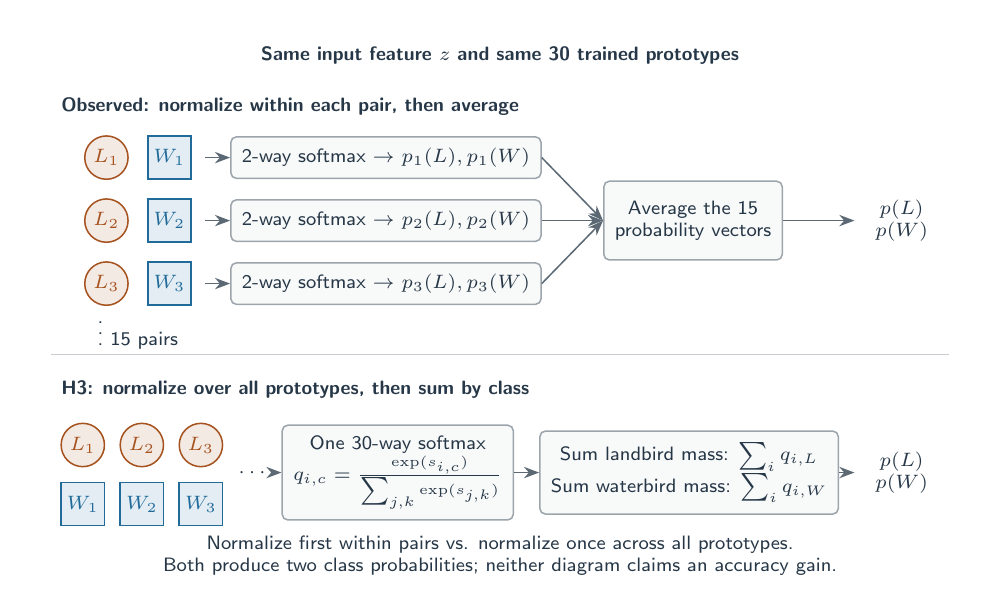
\begin{tikzpicture}[dpe diagram]
\path[use as bounding box] (-0.3,-6.6) rectangle (11.7,0.45);
\node[dpe heading] at (5.7,0.1) {Same input feature $z$ and same 30 trained prototypes};
\node[dpe heading,anchor=west] at (0,-0.55) {Observed: normalize within each pair, then average};
\foreach \i/\y in {1/-1.2,2/-2,3/-2.8} {
  \node[dpe land] (l\i) at (0.7,\y) {$L_{\i}$};
  \node[dpe water] (w\i) at (1.5,\y) {$W_{\i}$};
  \node[dpe box,minimum width=3.6cm] (s\i) at (4.25,\y)
    {2-way softmax $\to$ $p_{\i}(L),p_{\i}(W)$};
  \draw[dpe arrow] (1.95,\y) -- (s\i.west);
}
\node[dpe box,minimum height=1cm] (avg) at (8.15,-2) {Average the 15\\probability vectors};
\foreach \i in {1,2,3} {\draw[dpe arrow] (s\i.east) -- (avg.west);}
\node at (1.1,-3.35) {$\vdots$ 15 pairs};
\node[align=center] at (10.8,-2) {$p(L)$\\$p(W)$};
\draw[dpe arrow] (avg.east) -- (10.2,-2);
\draw[draw=dpeink!25] (0,-3.7) -- (11.4,-3.7);
\node[dpe heading,anchor=west] at (0,-4.15) {H3: normalize over all prototypes, then sum by class};
\foreach \i/\x in {1/0.4,2/1.15,3/1.9} {
  \node[dpe land] at (\x,-4.85) {$L_{\i}$};
  \node[dpe water] at (\x,-5.6) {$W_{\i}$};
}
\node at (2.55,-5.2) {$\cdots$};
\node[dpe box,minimum height=1.05cm] (joint) at (4.4,-5.2)
  {One 30-way softmax\\$q_{i,c}=\frac{\exp(s_{i,c})}{\sum_{j,k}\exp(s_{j,k})}$};
\draw[dpe arrow] (2.8,-5.2) -- (joint.west);
\node[dpe box,minimum height=1.05cm] (sum) at (8.1,-5.2)
  {Sum landbird mass: $\sum_i q_{i,L}$\\Sum waterbird mass: $\sum_i q_{i,W}$};
\draw[dpe arrow] (joint.east) -- (sum.west);
\node[align=center] at (10.8,-5.2) {$p(L)$\\$p(W)$};
\draw[dpe arrow] (sum.east) -- (10.2,-5.2);
\node[align=center] at (5.7,-6.25)
  {Normalize first within pairs vs. normalize once across all prototypes.\\Both produce two class probabilities; neither diagram claims an accuracy gain.};
\end{tikzpicture}

\caption{H3: give each head more prototypes while retaining the ensemble. The middle panel shows two prototypes per class in three illustrative heads; all 15 heads still output two class probabilities before averaging or H2 weighting. Circles are landbird prototypes, squares are waterbird prototypes, and subscripts identify their source heads in the existing pool. Each softmax is computed within the receiving head's subset, then probability mass is summed by class. The bottom panel shows global pooling as the special case of identical full-pool heads. No accuracy gain is assumed.}
\label{fig:dpe-h3}
\end{figure}

\section{Conclusion}
DPE and AutoBackSwap gave results close to their papers, and POTER still needs its test evaluation. Looking at AutoBackSwap's mistakes, we found that three species may be mislabeled in the dataset, and that they explain about 80\% of its $G_4$ errors. The three-seed H2 study found no WGA improvement from validation-selected global head weights over matched uniform averaging. Next steps are to investigate objective sensitivity and selection stability, and to evaluate conditional combiners; H1 and H3 remain open.
%
% ---- Bibliography ----
%
\begin{thebibliography}{8}
\sloppy
\bibitem{dpe}
To, M.N.N., Wilson, P.F.R., Nguyen, V., et al.: Diverse prototypical ensembles improve robustness to subpopulation shift. In: Proceedings of the 42nd International Conference on Machine Learning (2025). \url{https://arxiv.org/abs/2505.23027}

\bibitem{poter}
Jo, S.-H., et al.: Potentials from optimal transport for empirical reweighting. NeurIPS (2026). \url{https://arxiv.org/abs/2610.01028}

\bibitem{autobackswap}
Roder, C., Schweighofer, K.: Automated background swapping for robustness against spurious backgrounds. arXiv preprint arXiv:2606.32018 (2026). \url{https://arxiv.org/abs/2606.32018}

\bibitem{waterbirds}
Sagawa, S., Koh, P.W., Hashimoto, T.B., Liang, P.: Distributionally robust neural networks for group shifts: On the importance of regularization for worst-case generalization. In: International Conference on Learning Representations (2020).
\bibitem{stacking}
Wolpert, D.H.: Stacked generalization. Neural Networks 5(2), 241--259 (1992). \url{https://doi.org/10.1016/S0893-6080(05)80023-1}

\bibitem{mixtures}
Jacobs, R.A., Jordan, M.I., Nowlan, S.J., Hinton, G.E.: Adaptive mixtures of local experts. Neural Computation 3(1), 79--87 (1991). \url{https://doi.org/10.1162/neco.1991.3.1.79}
\end{thebibliography}
\end{document}
